\documentclass{article}




\usepackage{fullpage}
\usepackage{nopageno}
\usepackage{amsmath}
\usepackage{amsfonts}
\usepackage{graphicx}
\usepackage{framed}
\usepackage{algorithmic}
\usepackage{xcolor}

\definecolor{dark_red}{rgb}{0.5,0.0,0.0}
\definecolor{dark_green}{rgb}{0.0,0.5,0.0}
\definecolor{dark_blue}{rgb}{0.0,0.0,0.5}
\definecolor{blue}{rgb}{0.0,0.0,1.0}

\newcommand{\dr}[1]{\textcolor{dark_red}{#1}}
\newcommand{\dg}[1]{\textcolor{dark_green}{#1}}
\newcommand{\db}[1]{\textcolor{dark_blue}{#1}}
\newcommand{\blue}[1]{\textcolor{blue}{#1}}



\begin{document}

\section*{Systems of Equations}

A {\bf linear system} with the \(n\) variables \(x_1, x_2, ..., x_n\) and \(m\) equations has the following general form:
\[\left\{\begin{array}{c}
a_{1,1} x_1 + a_{1,2} x_2 + ... + a_{1,n} x_n = b_1 \\
a_{2,1} x_1 + a_{2,2} x_2 + ... + a_{2,n} x_n = b_2 \\
\vdots \\
a_{m,1} x_1 + a_{m,2} x_2 + ... + a_{m,n} x_n = b_m \\
\end{array}\right.\] 

The variables \(a_{1,1}\), \(a_{1,2}\), ..., \(a_{m,n}\) are fixed coefficients, and \(b_1\), \(b_2\), ..., \(b_m\) are fixed constants. 

The variables \(x_1\), \(x_2\), ..., \(x_n\) are the variables that are to be solved for. 

A linear system may have either \(1\), \(\infty\), or \(0\) solutions. When there are \(\infty\) many solutions, there may be multiple ``degrees of freedom", the set of solutions may form a multidimensional shape.

Below are given some very simple examples of linear systems:

\textbf{Examples}
\begin{itemize}
%%%%%%%%%%%%%%%%%%%%%%%
\item The simplest linear system consists of \(1\) variable and \(1\) equation. Consider for example the system: 
\[\left\{\begin{array}{c} 5x = 8 \end{array}\right.\]
The solution is clear, and is \(x = 8/5\). There is \(1\) solution.
%%%%%%%%%%%%%%%%%%%%%%%
\item Next consider a system with \(2\) variables and \(1\) equation. Consider for example the system:  
\[\left\{\begin{array}{c} 3x - 2y = 5 \end{array}\right.\]
Solving for \(x\) as a function of \(y\) gives:
\[3x - 2y = 5 \iff 3x = 5 + 2y \iff x = 5/3 + (2/3)y\]
\(y\) can be set to any value, and the value of \(x\) can be computed via \(x = 5/3 + (2/3)y\). There are \(\infty\) solutions, and they form a line in the \(xy\)-plane.
%%%%%%%%%%%%%%%%%%%%%%%
\item Next consider a system with \(1\) variable and \(2\) equations. Consider for example the system:  
\[\left\{\begin{array}{c} 3x = 2 \\ -6x = -4 \end{array}\right.\]
Solving the first equation for \(x\) gives:
\[3x = 2 \iff x = 2/3\]
Substituting this value for \(x\) into the second equation gives:
\[-6x = -4 \iff -6(2/3) = -4 \iff -4 = -4\]
This equation is always true, and hence brings no new information. There is \(1\) solution, namely \(x = 2/3\).
%%%%%%%%%%%%%%%%%%%%%%%
\item Consider the following system with \(1\) variable and \(2\) equations:  
\[\left\{\begin{array}{c} 2x = -5 \\ 4x = 3 \end{array}\right.\]
Solving the first equation for \(x\) gives:
\[2x = -5 \iff x = -5/2\]
Substituting this value for \(x\) into the second equation gives:
\[4x = 3 \iff 4(-5/2) = 3 \iff -10 = 3\]
This equation is always false, and the system can never be satisfied. There are \(0\) solutions.
%%%%%%%%%%%%%%%%%%%%%%%
\item Consider the following system with \(2\) variables and \(2\) equations:  
\[\left\{\begin{array}{c} 4x + 20y = 4 \\ -2x - 7y = -5 \end{array}\right.\]
Solving the first equation for \(x\) gives:
\[4x + 20y = 4 \iff 4x = 4 - 20y \iff x = 1 - 5y\]
Substituting this expression for \(x\) into the second equation gives:
\begin{align*}
& -2x - 7y = -5 \iff -2(1 - 5y) - 7y = -5 \iff (-2 + 10y) - 7y = -5 \\
& \iff -2 + 3y = -5 \iff 3y = -3 \iff y = -1
\end{align*}
With the knowledge that \(y = -1\), \(x = 1 - 5y = 6\). There is \(1\) solution, namely \(x = 6\) and \(y = -1\).
%%%%%%%%%%%%%%%%%%%%%%%
\item Consider the following system with \(2\) variables and \(2\) equations:  
\[\left\{\begin{array}{c} 5x - 35y = 10 \\ -3x + 21y = -6 \end{array}\right.\]
Solving the first equation for \(x\) gives:
\[5x - 35y = 10 \iff 5x = 10 + 35y \iff x = 2 + 7y\]
Substituting this expression for \(x\) into the second equation gives:
\begin{align*}
& -3x + 21y = -6 \iff -3(2 + 7y) + 21y = -6 \iff (-6 - 21y) + 21y = -6 \\
& \iff -6 = -6  
\end{align*}
The second equation provides no new information. \(y\) can be set to any value, and the value of \(x\) can be computed via \(x = 2 + 7y\). There are \(\infty\) solutions, and they form a line in the \(xy\)-plane.
%%%%%%%%%%%%%%%%%%%%%%%
\item Consider the following system with \(2\) variables and \(2\) equations:  
\[\left\{\begin{array}{c} 5x - 35y = -5 \\ -3x + 21y = 1 \end{array}\right.\]
Solving the first equation for \(x\) gives:
\[5x - 35y = -5 \iff 5x = -5 + 35y \iff x = -1 + 7y\]
Substituting this expression for \(x\) into the second equation gives:
\begin{align*}
& -3x + 21y = 1 \iff -3(-1 + 7y) + 21y = 1 \iff (3 - 21y) + 21y = 1 \\
& \iff 3 = 1  
\end{align*}
The second equation is always false, and the system can never be satisfied. There are \(0\) solutions.
\end{itemize}

Consider the general \(2\) variable, \(2\) equation system:
\[\left\{\begin{array}{c}
a_1 x + b_1 y = c_1 \\
a_2 x + b_2 y = c_2
\end{array}\right.\]
The equations \(a_1 x + b_1 y = c_1\) and \(a_2 x + b_2 y = c_2\) each define a line. Regarding the sets of possible solutions, there are \(3\) alternatives.

\begin{tabular}{cc}
\parbox{0.5\textwidth}{
When there is {\bf \(1\) solution}, the lines formed by the equations \(a_1 x + b_1 y = c_1\) and \(a_2 x + b_2 y = c_2\) are {\bf not parallel} and hence intersect at a common point. 
} & \parbox{0.5\textwidth}{
\includegraphics[width = 0.4\textwidth]{2_variable_system_1_solution}
} 
\end{tabular}

\begin{tabular}{cc}
\parbox{0.5\textwidth}{
When there are {\bf \(\infty\) solutions}, the lines formed by the equations \(a_1 x + b_1 y = c_1\) and \(a_2 x + b_2 y = c_2\) are {\bf the same line}. 
} & \parbox{0.5\textwidth}{
\includegraphics[width = 0.4\textwidth]{2_variable_system_inf_solutions}
} 
\end{tabular}

\begin{tabular}{cc}
\parbox{0.5\textwidth}{
When there are {\bf \(0\) solutions}, the lines formed by the equations \(a_1 x + b_1 y = c_1\) and \(a_2 x + b_2 y = c_2\) are {\bf parallel, but not the same line}. 
} & \parbox{0.5\textwidth}{
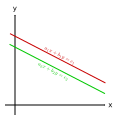
\includegraphics[width = 0.4\textwidth]{2_variable_system_0_solutions}
} 
\end{tabular}

Consider the general \(3\) variable, \(3\) equation system:
\[\left\{\begin{array}{c}
a_1 x + b_1 y + c_1 z = d_1 \\
a_2 x + b_2 y + c_2 z = d_2 \\
a_3 x + b_3 y + c_3 z = d_3
\end{array}\right.\]

Each equation defines a plane. Regarding the sets of possible solutions, there are \(4\) alternatives, with multiple scenarios present in each alternative.

\begin{tabular}{cc}
\parbox{0.4\textwidth}{
When there is {\bf \(1\) solution}, the no \(2\) planes are parallel. There are \(3\) intersection lines formed by the intersection of each pair of planes, and no \(2\) intersection lines are parallel either. 
} & \parbox{0.6\textwidth}{
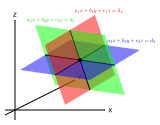
\includegraphics[width = 0.6\textwidth]{3_variable_system_1_solution}
}
\end{tabular}

The next scenario is {\bf \(\infty\) solutions with \(1\) degree of freedom}. In this case, the common intersection forms a line. There are two scenarios. One scenario (shown on the left) is where no \(2\) planes are parallel, and the intersection lines formed by the intersection of each pair of planes are all the same line. The other scenario (shown on the right) is where \(2\) of the planes are the same plane, and the remaining plane is not parallel to the other \(2\) planes.

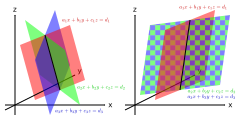
\includegraphics[width = 0.9\textwidth]{3_variable_system_inf_solutions}  

\begin{tabular}{cc}
\parbox{0.4\textwidth}{
When there is {\bf \(\infty\) solutions with \(2\) degrees of freedom}, all \(3\) planes are the same plane. In this case, the common intersection is a plane, namely the common plane from all \(3\) equations. 
} & \parbox{0.6\textwidth}{

\includegraphics[width = 0.6\textwidth]{3_variable_system_inf2_solutions}
}
\end{tabular}

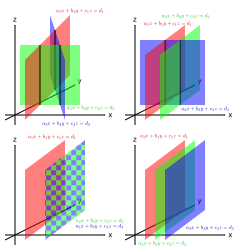
\includegraphics[width = 0.9\textwidth]{3_variable_system_0_solutions} 

A linear system is {\bf consistent} if there is at least 1 solution, and {\bf inconsistent} if there are no solutions. 



\section*{Augmented matrices}

To better represent a linear system, and the process of solving a linear system, the linear system will be shorthanded via an array of coefficients referred to as an {\bf augmented matrix}. 

The augmented matrix of the linear system:

\[\left\{\begin{array}{c}
a_{1,1} x_1 + a_{1,2} x_2 + ... + a_{1,n} x_n = b_1 \\
a_{2,1} x_1 + a_{2,2} x_2 + ... + a_{2,n} x_n = b_2 \\
\vdots \\
a_{m,1} x_1 + a_{m,2} x_2 + ... + a_{m,n} x_n = b_m \\
\end{array}\right.\] 
is
\[\left[\begin{array}{cccc|c}
a_{1,1} & a_{1,2} & \cdots & a_{1,n} & b_1 \\   
a_{2,1} & a_{2,2} & \cdots & a_{2,n} & b_2 \\   
\vdots & \vdots & \ddots & \vdots & \vdots \\ 
a_{m,1} & a_{m,2} & \cdots & a_{m,n} & b_m 
\end{array}\right]\]
The rows are indexed from top to bottom, and each row corresponds to an equation. The columns are indexed from left to right, and each column, save for the last ``augmented column", corresponds to a variable. The last ``augmented column", separated from the rest of the matrix via a vertical line, contains the constant terms found on the right hand side of the linear equations.

\textbf{Examples:}
\begin{itemize}
%%%%%%%%%%%%%%%%%%%%%%%
\item 
\[\left\{\begin{array}{c}
5x_1 - 35x_2 + 15x_3 = -35 \\
-x_1 + 2x_2 - 13x_3 = 12 \\
2x_1 - 11x_2 + 20x_3 = -25
\end{array}\right. 
\quad\iff\quad 
\left[\begin{array}{ccc|c}
5 & -35 & 15 & -35 \\
-1 & 2 & -13 & 12 \\
2 & -11 & 20 & -25
\end{array}\right]\]
%%%%%%%%%%%%%%%%%%%%%%%
\item 
\[\left\{\begin{array}{c}
-2x_1 - 8x_2 = -54 \\
-x_1 - 7x_2 = -45 \\
x_1 + 2x_2 = 8
\end{array}\right. 
\quad\iff\quad 
\left[\begin{array}{cc|c}
-2 & -8 & -54 \\
-1 & -7 & -45 \\
1 & 2 & 8 
\end{array}\right]\]
%%%%%%%%%%%%%%%%%%%%%%%
\item 
\[\left\{\begin{array}{c}
-3x_1 - 15x_2 + 9x_3 = -18 \\
2x_1 + 6x_2 + 2x_3 = -8 \\
x_1 + 2x_2 + 3x_3 = -9
\end{array}\right. 
\quad\iff\quad 
\left[\begin{array}{ccc|c}
-3 & -15 & 9 & -18\\
2 & 6 & 2 & -8 \\
1 & 2 & 3 & -9 
\end{array}\right]\]
%%%%%%%%%%%%%%%%%%%%%%%
\item 
\[\left\{\begin{array}{c}
3x_1 - 6x_2 + 9x_3 = -3 \\
-6x_1 + 12x_2 - 13x_3 = 4 
\end{array}\right. 
\quad\iff\quad 
\left[\begin{array}{ccc|c}
3 & -6 & 9 & -3 \\ 
-6 & 12 & -13 & 4 
\end{array}\right]\]
%%%%%%%%%%%%%%%%%%%%%%%
\item 
\[\left\{\begin{array}{c}
x_1 - x_3 = 4 \\
x_4 - 6x_2 = -1  
\end{array}\right. 
\quad\iff\quad 
\left[\begin{array}{cccc|c}
1 & 0 & -1 & 0 & 4 \\ 
0 & -6 & 0 & 1 & -1 
\end{array}\right]\]
\end{itemize}

Given a system of equations, the following {\bf elementary row operations} are applied to the augmented matrix in the process of solving the system of equations. There are \(3\) types of elementary row operations.

\vspace{5mm}

%%%%%%
{\bf Row replacement:} Given two equations, a multiple of one equation can be added to another equation without affecting the truth or falsity of the system. Let \(i\) and \(j\) index two different equations/rows, and let \(k\) be an arbitrary nonzero constant: 
\begin{align*}
& \left\{\begin{array}{c}
\vdots \\
a_{i,1} x_1 + a_{i,2} x_2 + ... + a_{i,n} x_n = b_i \\
\vdots \\
a_{j,1} x_1 + a_{j,2} x_2 + ... + a_{j,n} x_n = b_j \\
\vdots
\end{array}\right. \\
& \iff
\left\{\begin{array}{c}
\vdots \\
a_{i,1} x_1 + a_{i,2} x_2 + ... + a_{i,n} x_n = b_i \\
\vdots \\
(a_{j,1} + ka_{i,1}) x_1 + (a_{j,2} + ka_{i,2}) x_2 + ... + (a_{j,n} + ka_{i,n}) x_n = b_j + kb_i \\
\vdots
\end{array}\right.
\end{align*}

In terms of augmented matrices, this operation is:
\[\left[\begin{array}{cccc|c}
\vdots & \vdots &  & \vdots & \vdots \\   
a_{i,1} & a_{i,2} & \cdots & a_{i,n} & b_i \\   
\vdots & \vdots &  & \vdots & \vdots \\ 
a_{j,1} & a_{j,2} & \cdots & a_{j,n} & b_j \\
\vdots & \vdots &  & \vdots & \vdots
\end{array}\right] 
\xrightarrow{R_j \rightarrow R_j + kR_i} 
\left[\begin{array}{cccc|c}
\vdots & \vdots &  & \vdots & \vdots \\   
a_{i,1} & a_{i,2} & \cdots & a_{i,n} & b_i \\   
\vdots & \vdots &  & \vdots & \vdots \\ 
a_{j,1} + ka_{i, 1} & a_{j,2} + ka_{i, 2} & \cdots & a_{j,n} + ka_{i,n} & b_j + kb_i \\
\vdots & \vdots &  & \vdots & \vdots
\end{array}\right]\]
Here, the notation \(R_j \rightarrow R_j + kR_i\) reads as replace row \(j\) with row \(j\) plus \(k\) times row \(i\). Note that despite the above equation, row \(j\) may be above row \(i\).

\vspace{5mm}

%%%%%%
{\bf Row scaling:} Given a single equation, multiplying both sides by the same nonzero constant has no no effect on the truth or falsity of the system. Let \(i\) index an arbitrary row, and let \(k\) be an arbitrary nonzero constant:
\[\left\{\begin{array}{c}
\vdots \\   
a_{i,1} x_1 + a_{i,2} x_2 + ... + a_{i,n} x_n = b_i \\   
\vdots 
\end{array}\right. 
\iff 
\left\{\begin{array}{c}
\vdots \\   
k a_{i,1} x_1 + k a_{i,2} x_2 + ... + k a_{i,n} x_n = k b_i \\   
\vdots 
\end{array}\right.\]

In terms of augmented matrices, this operation is:
\[\left[\begin{array}{cccc|c}
\vdots & \vdots &  & \vdots & \vdots \\   
a_{i,1} & a_{i,2} & \cdots & a_{i,n} & b_i \\   
\vdots & \vdots &  & \vdots & \vdots 
\end{array}\right] 
\xrightarrow{R_i \rightarrow kR_i} 
\left[\begin{array}{cccc|c}
\vdots & \vdots &  & \vdots & \vdots \\   
k a_{i,1} & k a_{i,2} & \cdots & k a_{i,n} & k b_i \\   
\vdots & \vdots &  & \vdots & \vdots 
\end{array}\right]\]
Here, the notation \(R_i \rightarrow kR_i\) reads as multiply row \(i\) by \(k\).

\vspace{5mm}

%%%%%%
{\bf Row swapping:} Given two equations, the two equations can be swapped around without affecting the truth or falsity of the system. Let \(i\) and \(j\) index two different equations/rows.
\[\left\{\begin{array}{c}
\vdots \\   
a_{i,1} x_1 + a_{i,2} x_2 + ... + a_{i,n} x_n = b_i \\   
\vdots \\ 
a_{j,1} x_1 + a_{j,2} x_2 + ... + a_{j,n} x_n = b_j \\
\vdots 
\end{array}\right. 
\iff 
\left\{\begin{array}{c}
\vdots \\   
a_{j,1} x_1 + a_{j,2} x_2 + ... + a_{j,n} x_n = b_j \\   
\vdots \\ 
a_{i,1} x_1 + a_{i,2} x_2 + ... + a_{i,n} x_n = b_i \\
\vdots 
\end{array}\right.\]

In terms of augmented matrices, this operation is:
\[\left[\begin{array}{cccc|c}
\vdots & \vdots &  & \vdots & \vdots \\   
a_{i,1} & a_{i,2} & \cdots & a_{i,n} & b_i \\   
\vdots & \vdots &  & \vdots & \vdots \\ 
a_{j,1} & a_{j,2} & \cdots & a_{j,n} & b_j \\
\vdots & \vdots &  & \vdots & \vdots
\end{array}\right] 
\xrightarrow{R_i \leftrightarrow R_j} 
\left[\begin{array}{cccc|c}
\vdots & \vdots &  & \vdots & \vdots \\   
a_{j,1} & a_{j,2} & \cdots & a_{j,n} & b_j \\   
\vdots & \vdots &  & \vdots & \vdots \\ 
a_{i,1} & a_{i,2} & \cdots & a_{i,n} & b_i \\
\vdots & \vdots &  & \vdots & \vdots
\end{array}\right]\]
Here, the notation \(R_i \leftrightarrow R_j\) reads as swap rows \(i\) and \(j\).



\section*{Gaussian elimination}

Gaussian elimination refers to the process of solving systems of equations by applying the elementary row operations to the augmented matrix. The goal is to first convert the augmented matrix to {\bf row echelon form}, and then to {\bf row reduced echelon form}. Once the augmented matrix has been converted to row reduced echelon form, the system of equations has been solved.

The first nonzero entry of a row in a matrix is referred to as a {\bf pivot}.

A matrix is in {\bf row echelon form} if and only if the following properties hold:
\begin{itemize}
\item All zero rows are at the bottom of the matrix. 
\item For every nonzero row that is not the top row, the pivot of the row is in a column that is strictly to the right of the pivot of the row above it.
\end{itemize}

The following example matrices are in row echelon form. Each \(*\) denotes an arbitrary value, and each \(X\) denotes an arbitrary nonzero value.

\begin{tabular}{cccc}
\(\left[\begin{array}{cc|c}
0 & 0 & 0 \\
0 & 0 & 0
\end{array}\right]\)
&
\(\left[\begin{array}{ccc|c}
X & * & * & * \\
0 & X & * & * \\
0 & 0 & X & *
\end{array}\right]\)
&
\(\left[\begin{array}{cccccc|c}
0 & X & * & * & * & * & * \\
0 & 0 & 0 & X & * & * & * \\
0 & 0 & 0 & 0 & X & * & * \\
0 & 0 & 0 & 0 & 0 & 0 & X
\end{array}\right]\)
& 
\(\left[\begin{array}{cccc|c}
X & * & * & * & * \\
0 & 0 & X & * & * \\
0 & 0 & 0 & X & * \\
0 & 0 & 0 & 0 & 0 \\
0 & 0 & 0 & 0 & 0
\end{array}\right]\)
\end{tabular}

A matrix is in {\bf row reduced echelon form} (often simply referred to as row reduced form) if and only if the following properties hold:
\begin{itemize}
\item The matrix is in row echelon form. 
\item Every pivot has a value of \(1\). 
\item Each column that contains a pivot contains \(0\)'s in all other entries. 
\end{itemize} 

The following example matrices are in row reduced echelon form. Each \(*\) denotes an arbitrary value, and each \(X\) denotes an arbitrary nonzero value.

\begin{tabular}{cccc}
\(\left[\begin{array}{cc|c}
0 & 0 & 0 \\
0 & 0 & 0
\end{array}\right]\)
&
\(\left[\begin{array}{ccc|c}
1 & 0 & 0 & * \\
0 & 1 & 0 & * \\
0 & 0 & 1 & *
\end{array}\right]\)
&
\(\left[\begin{array}{cccccc|c}
0 & 1 & * & 0 & 0 & * & 0 \\
0 & 0 & 0 & 1 & 0 & * & 0 \\
0 & 0 & 0 & 0 & 1 & * & 0 \\
0 & 0 & 0 & 0 & 0 & 0 & 1
\end{array}\right]\)
& 
\(\left[\begin{array}{cccc|c}
1 & * & 0 & 0 & * \\
0 & 0 & 1 & 0 & * \\
0 & 0 & 0 & 1 & * \\
0 & 0 & 0 & 0 & 0 \\
0 & 0 & 0 & 0 & 0
\end{array}\right]\)
\end{tabular}

When a system has been converted to row reduced echelon form, the solution becomes clear:
\begin{itemize}
\item If the last column (the augmented column) contains a pivot, then the associated equation is \(0 = 1\) which is a contradiction. There are {\bf no solutions}, and the linear system is {\bf inconsistent}. If the last column does not contain a pivot, then there {\bf are solutions}, and the system is {\bf consistent}. 
\item Each variable that corresponds to a column that does not contain a pivot is referred to as a {\bf free variable}. The values of free variables can be arbitrarily set, and there will still exist a solution.
\item Each variable that corresponds to a column that contains a pivot is referred to as a {\bf bound variable}, also referred to as a {\bf leading variable}, is a variable whose value is either fixed or determined by the free variables. 
\end{itemize}

Consider for example the row reduced matrix:
\[\left[\begin{array}{ccc|c}
1 & -7 & 0 & 0 \\
0 & 0 & 1 & 0 \\
0 & 0 & 0 & 1 \\
0 & 0 & 0 & 0
\end{array}\right]\]
There is a pivot in the last column, so the third row corresponds to the equation \(0 = 1\). This is a contradiction and the system therefore has {\bf no solutions}.

\vspace{1mm}

Consider now for example the row reduced matrix:
\[\left[\begin{array}{cccccc|c}
0 & 1 & 3 & 0 & 0 & -4 & 2 \\
0 & 0 & 0 & 1 & 0 & 2 & 1 \\
0 & 0 & 0 & 0 & 1 & -1 & -5 \\
0 & 0 & 0 & 0 & 0 & 0 & 0
\end{array}\right]\]
There are \(6\) variables, \(x_1\), \(x_2\), \(x_3\), \(x_4\), \(x_5\), and \(x_6\). There is no pivot in the last column so the system is consistent. The system of equations that corresponds to this augmented matrix is:
\[\left\{\begin{array}{c}
x_2 + 3x_3 - 4x_6 = 2 \\
x_4 + 2x_6 = 1 \\
x_5 - x_6 = -5 \\
0 = 0
\end{array}\right.\] 
Variables \(x_1\), \(x_3\) and \(x_6\) are the free variables, and can be arbitrarily set to any value. Variables \(x_2\), \(x_4\), and \(x_5\) are the bound variables which are functions of the free variables. 
The first equation yields \(x_2 = 2 - 3x_3 + 4x_6\), the second equation yields \(x_4 = 1 - 2x_6\), the third equation yields \(x_5 = -5 + x_6\), and the fourth equation gives no information. Any arbitrary solution can generated by first choosing the values of \(x_1\), \(x_3\), and \(x_6\): \(x_1 = s\), \(x_3 = t\), and \(x_6 = u\) where \(s\), \(t\), and \(u\) are arbitrary. The values of the bound variables are \(x_2 = 2 - 3t + 4u\), \(x_4 = 1 - 2u\), and \(x_5 = -5 + u\). The solution is often presented as a linear combination of constant vectors:

\[\begin{bmatrix} x_1 \\ x_2 \\ x_3 \\ x_4 \\ x_5 \\ x_6 \end{bmatrix} = \begin{bmatrix} s \\ 2 - 3t + 4u \\ t \\ 1 - 2u \\ -5 + u \\ u \end{bmatrix} 
= \begin{bmatrix} 0 \\ 2 \\ 0 \\ 1 \\ -5 \\ 0 \end{bmatrix} + s\begin{bmatrix} 1 \\ 0 \\ 0 \\ 0 \\ 0 \\ 0 \end{bmatrix} + t\begin{bmatrix} 0 \\ -3 \\ 1 \\ 0 \\ 0 \\ 0 \end{bmatrix} + u\begin{bmatrix} 0 \\ 4 \\ 0 \\ -2 \\ 1 \\ 1 \end{bmatrix}\] 

As can be seen, the number of free variables determines how many ``dimensions" or ``degrees of freedom" that the set of solutions has.

How to convert a matrix to row reduced form? Now will be described the process of Gaussian elimination.

\begin{itemize} 
\item Let \(m\) denote the number of equations. 
\item Let \(n\) denote the number of variables. 
\item Let \(a[i,j]\) where \(1 \leq i \leq m\) and \(1 \leq j \leq n\) denote the coefficient of \(x_j\) in equation \(i\). 
\item Let \(b[i]\) where \(1 \leq i \leq m\) denote the the constant on the right hand side of the \(i^{\text{th}}\) equation. 
\item The augmented matrix itself will be denoted by \(A\), and has \(m\) rows and \(n + 1\) columns. In the augmented matrix, \(a[i,j]\) is the entry on row \(i\) and column \(j\). For completeness, since the augmented column is the \((n + 1)^{\text{th}}\) column of \(A\), the entry \(b[i]\) will also be referenced by \(a[i, n+1]\): \(a[i,n+1] = b[i]\). 
\end{itemize}

\[A = \left[\begin{array}{cccc|c}
a[1,1] & a[1,2] & \cdots & a[1,n] & b[1] \\ 
a[2,1] & a[2,2] & \cdots & a[2,n] & b[2] \\
\vdots & \vdots & \ddots & \vdots & \vdots \\
a[m,1] & a[m,2] & \cdots & a[m,n] & b[m] 
\end{array}\right]\]

%To determine if a matrix is in {\bf row echelon form}, let \(\text{pivot}[i]\) denote the column index of the first nonzero entry of row \(i\). Let \(\text{has\_pivot}[i]\) be a condition that is ``true" if and only if row \(i\) has a pivot and is not all \(0\)'s.
%%If row \(i\) is all \(0\)'s, then \(\text{pivot}[i]\) defaults to \(+\infty\). By default \(+\infty < +\infty\). 
%
%A matrix is in {\bf row echelon form} if and only if for all row indices \(i\) one of the following is true: 
%\[\left\{\begin{array}{cc}
%& i = 1 \\
%\text{OR} & \big( \text{has\_pivot}[i-1] \;\text{AND}\; \text{has\_pivot}[i] \;\text{AND}\; (\text{pivot}[i-1] < \text{pivot}[i]) \big) \\
%\text{OR} & \big( \text{has\_pivot}[i-1] \;\text{AND}\; (\text{NOT}\; \text{has\_pivot}[i]) \big) \\
%\text{OR} & \big( (\text{NOT}\; \text{has\_pivot}[i-1]) \;\text{AND}\; (\text{NOT}\; \text{has\_pivot}[i]) \big)
%\end{array}\right.\]

The following algorithm describes the process of ``Gaussian elimination". The elementary row operations will change the values of the matrix entries \(a[i,j]\).

\begin{algorithmic}
\STATE \texttt{// The matrix will first be converted to row echelon form.}
\STATE Let \(i = 1\) ~~~ \texttt{// i will track the row that is currently under consideration.}
\STATE Let \(j = 1\) ~~~ \texttt{// j will track the column that is currently under consideration.}
\WHILE{\(i \leq m \;\;\text{AND}\;\; j \leq n\)}
	\STATE \texttt{// Check if there are any nonzero entries in column j starting from index i and downwards. The first nonzero entry encountered will be the pivot of column j.}
	\STATE Let \(i_2 = i\)
	\STATE Let \(\text{pivot\_found\_flag} = \textbf{false}\)
	\WHILE{\((\text{pivot\_found\_flag} = \textbf{false})\;\;\text{AND}\;\;(i_2 \leq m)\)} 
		\IF{\(a[i_2, j] \neq 0\)}
			\STATE \texttt{// A pivot for column j has been found. Now swap the rows so the pivot is at entry (i, j).}
			\STATE Change \(\text{pivot\_found\_flag}\) to \(\textbf{true}\)
			\STATE {\bf Swap rows \(i\) and \(i_2\).} ~~~ \texttt{// No swap occurs if the rows are the same.}
		\ELSE
			\STATE Change \(i_2\) to \(i_2 + 1\)
		\ENDIF
	\ENDWHILE
	\IF{\(\text{pivot\_found\_flag} = \textbf{true}\)}
		\STATE \texttt{// Eliminate all entries beneath entry (i, j) by adding the appropriate multiples of row i.}
		\STATE Let \(i_2 = i + 1\)
		\WHILE{\(i_2 \leq m\)}
			\STATE Let \(k = -\frac{a[i_2,j]}{a[i,j]}\)
			\STATE {\bf Add \(k\) times row \(i\) to row \(i_2\).}
			\STATE Change \(i_2\) to \(i_2 + 1\)
		\ENDWHILE
		\STATE Change \(i\) to \(i + 1\) ~~~ \texttt{// Advance to the next row now that a pivot has been found and used.}
	\ENDIF
	\STATE Change \(j\) to \(j + 1\)
	\STATE \texttt{// The loop will exit when \(i\) or \(j\) leaves the range of valid indices.}
\ENDWHILE
\STATE \texttt{// The matrix is now in row echelon form. A conversion to row reduced echelon form will now occur.}
\STATE Let \(i = m\) 
\WHILE{\(i \geq 1\)}
%	\STATE \texttt{Find the pivot in row i.}
%	\STATE Let \(\text{pivot\_found\_flag} = \textbf{false}\)
%	\STATE Let \(j = 1\)
%	\WHILE{\((\text{pivot\_found\_flag} = \textbf{false}) \;\;\text{AND}\;\; (j \leq n)\)}
%		\IF{\(a[i, j] \neq 0\)}
%			\STATE Change \(\text{pivot\_found\_flag}\) to \(\textbf{true}\) 
%			\STATE Let \(\text{pivot\_column\_index} = j\)
%		\ELSE
%			\STATE Change \(j\) to \(j + 1\)
%		\ENDIF
%	\ENDWHILE
% 	\IF{\(\text{pivot\_found\_flag} = \textbf{true}\)}
%		\STATE \texttt{// Eliminate all entries above entry (i, pivot\_column\_index) by adding the appropriate multiples of row i.}
%		\STATE Let \(i_2 = i - 1\)
%	\ENDIF
	\IF{there exists a pivot in row \(i\)}
		\STATE Let \(\text{pivot\_column\_index}\) denote the pivot's column index.
		\STATE \texttt{// The pivot will be made 1 by dividing row i by the pivot's value}
		\STATE {\bf Multiply row \(i\) by \(\frac{1}{a[i,\textnormal{pivot\_column\_index}]}\)}
		\STATE \texttt{// Eliminate all entries above entry (i, pivot\_column\_index) by adding the appropriate multiples of row i.}
		\STATE Let \(i_2 = i - 1\)
		\WHILE{\(i_2 \geq 1\)}
			\STATE {\bf Add \(-a[i_2, \textnormal{pivot\_column\_index}]\) times row \(i\) to row \(i_2\).}
			\STATE Change \(i_2\) to \(i_2 - 1\)
		\ENDWHILE
	\ENDIF
	\STATE Change \(i\) to \(i - 1\)
\ENDWHILE
\STATE \texttt{// The matrix is now in row reduced echelon form.}
\end{algorithmic}

\vspace{1cm}

\textbf{Abstract Example:}

Now will be given some abstract examples to illustrate the overall process of Gaussian elimination. Each \(*\) denotes an arbitrary value, and each \(X\) denotes an arbitrary nonzero value. Consider the arbitrary augmented matrix:
\[\left[\begin{array}{ccccc|c}
0 & * & * & * & * & * \\
X & * & * & * & * & * \\
* & * & * & * & * & * \\
* & * & * & * & * & * \\
* & * & * & * & * & * 
\end{array}\right]\]
The first step is to convert the matrix to row echelon form. There are nonzero entries in the first column, so there will be a pivot in the first column. This pivot must belong to row \(1\), so rows \(1\) and \(2\) will be swapped:
\[\xrightarrow{\begin{array}{c} R_1 \leftrightarrow R_2 \end{array}} \left[\begin{array}{ccccc|c}
X & * & * & * & * & * \\
0 & * & * & * & * & * \\
* & * & * & * & * & * \\
* & * & * & * & * & * \\
* & * & * & * & * & * 
\end{array}\right]\]
The pivots of all rows beneath row \(1\) must be strictly to the right of column \(1\), so appropriate multiples of row \(1\) will be added to rows \(3\), \(4\), and \(5\) so all entries beneath the row \(1\) pivot are \(0\):
\[\xrightarrow{\begin{array}{c} R_3 \rightarrow R_3 + *R_1 \\ R_4 \rightarrow R_4 + *R_1 \\ R_5 \rightarrow R_5 + *R_1 \end{array}} \left[\begin{array}{ccccc|c}
X & * & * & * & * & * \\
0 & \blue{X} & * & * & * & * \\
0 & * & * & * & * & * \\
0 & * & * & * & * & * \\
0 & * & * & * & * & * 
\end{array}\right]\]
Any symbols highlighted in \blue{blue} have arisen by chance. The pivot for row \(2\) is in column \(2\), and all entries beneath the pivot need to be made \(0\) be adding appropriate multiples of row \(2\) to rows \(3\), \(4\), and \(5\):
\[\xrightarrow{\begin{array}{c} R_3 \rightarrow R_3 + *R_2 \\ R_4 \rightarrow R_4 + *R_2 \\ R_5 \rightarrow R_5 + *R_2 \end{array}} \left[\begin{array}{ccccc|c}
X & * & * & * & * & * \\
0 & X & * & * & * & * \\
0 & 0 & \blue{0} & \blue{0} & \blue{0} & \blue{0} \\
0 & 0 & \blue{0} & \blue{X} & * & * \\
0 & 0 & \blue{0} & * & * & * 
\end{array}\right]\]
The remainder of column \(3\) is all \(0\)'s, so there is no pivot in column \(3\). The remainder of column \(4\) contains a nonzero entry in row \(4\) which will be moved to be the pivot of row \(3\) by swapping rows \(3\) and \(4\):
\[\xrightarrow{\begin{array}{c} R_3 \leftrightarrow R_4 \end{array}} \left[\begin{array}{ccccc|c}
X & * & * & * & * & * \\
0 & X & * & * & * & * \\
0 & 0 & 0 & X & * & * \\
0 & 0 & 0 & 0 & 0 & 0 \\
0 & 0 & 0 & * & * & * 
\end{array}\right]\]
The pivot for row \(3\) is in column \(4\), and all entries beneath the pivot need to be made \(0\) be adding an appropriate multiple of row \(3\) to row \(5\):
\[\xrightarrow{\begin{array}{c} R_5 \rightarrow R_5 + *R_3 \end{array}} \left[\begin{array}{ccccc|c}
X & * & * & * & * & * \\
0 & X & * & * & * & * \\
0 & 0 & 0 & X & * & * \\
0 & 0 & 0 & 0 & 0 & 0 \\
0 & 0 & 0 & 0 & \blue{0} & \blue{0} 
\end{array}\right]\]

The matrix in row echelon form is hence:
\[\left[\begin{array}{ccccc|c}
X & * & * & * & * & * \\
0 & X & * & * & * & * \\
0 & 0 & 0 & X & * & * \\
0 & 0 & 0 & 0 & 0 & 0 \\
0 & 0 & 0 & 0 & 0 & 0 
\end{array}\right]\]
Since there is no pivot in the rightmost column, there are solutions to this system. The task is now to convert the matrix to row reduced echelon form. Working backwards from the rightmost pivot to the leftmost pivot, we first make the row \(3\) pivot \(1\) by multiplying row \(3\) by an appropriate constant:
\[\xrightarrow{\begin{array}{c} R_3 \rightarrow *R_3 \end{array}} \left[\begin{array}{ccccc|c}
X & * & * & * & * & * \\
0 & X & * & * & * & * \\
0 & 0 & 0 & 1 & * & * \\
0 & 0 & 0 & 0 & 0 & 0 \\
0 & 0 & 0 & 0 & 0 & 0 
\end{array}\right]\]
The next step is to add appropriate multiples of row \(3\) to rows \(1\) and \(2\) to create \(0\)'s above the row \(3\) pivot:
\[\xrightarrow{\begin{array}{c} R_1 \rightarrow R_1 + *R_3 \\ R_2 \rightarrow R_2 + *R_3 \end{array}} \left[\begin{array}{ccccc|c}
X & * & * & 0 & * & * \\
0 & X & * & 0 & * & * \\
0 & 0 & 0 & 1 & * & * \\
0 & 0 & 0 & 0 & 0 & 0 \\
0 & 0 & 0 & 0 & 0 & 0 
\end{array}\right]\]
The row \(2\) pivot is to be made \(1\) by multiplying row \(2\) by an appropriate constant: 
\[\xrightarrow{\begin{array}{c} R_2 \rightarrow *R_2 \end{array}} \left[\begin{array}{ccccc|c}
X & * & * & 0 & * & * \\
0 & 1 & * & 0 & * & * \\
0 & 0 & 0 & 1 & * & * \\
0 & 0 & 0 & 0 & 0 & 0 \\
0 & 0 & 0 & 0 & 0 & 0 
\end{array}\right]\]
The entries above the row \(2\) pivot are to be made \(0\) by adding an appropriate multiple of row \(2\) to row \(1\):
\[\xrightarrow{\begin{array}{c} R_1 \rightarrow R_1 + *R_2 \end{array}} \left[\begin{array}{ccccc|c}
X & 0 & * & 0 & * & * \\
0 & 1 & * & 0 & * & * \\
0 & 0 & 0 & 1 & * & * \\
0 & 0 & 0 & 0 & 0 & 0 \\
0 & 0 & 0 & 0 & 0 & 0 
\end{array}\right]\]
Lastly, the row \(1\) pivot is made \(1\) by multiplying row \(1\) by an appropriate constant:
\[\xrightarrow{\begin{array}{c} R_1 \rightarrow *R_1 \end{array}} \left[\begin{array}{ccccc|c}
1 & 0 & * & 0 & * & * \\
0 & 1 & * & 0 & * & * \\
0 & 0 & 0 & 1 & * & * \\
0 & 0 & 0 & 0 & 0 & 0 \\
0 & 0 & 0 & 0 & 0 & 0 
\end{array}\right]\]
The matrix is finally in row reduced echelon form.


\textbf{Examples:}

Now will be given some concrete examples with actual numbers.
\begin{itemize}
%%%%%%%%%%%%%%%%%%%%%%%%%
\item 
The system 
\[\left\{\begin{array}{c}
5x_1 - 35x_2 + 15x_3 = -35 \\
-x_1 + 2x_2 - 13x_3 = 12 \\
2x_1 - 11x_2 + 20x_3 = -25
\end{array}\right.\]
will be solved via Gaussian elimination. The first step is to convert to row echelon form:
\begin{align*}
& \left[\begin{array}{ccc|c}
5 & -35 & 15 & -35 \\
-1 & 2 & -13 & 12 \\
2 & -11 & 20 & -25
\end{array}\right]
\xrightarrow{\begin{array}{c} R_2 \rightarrow R_2 + (1/5)R_1 \\ R_3 \rightarrow R_3 - (2/5)R_1 \end{array}}
\left[\begin{array}{ccc|c}
5 & -35 & 15 & -35 \\
0 & -5 & -10 & 5 \\
0 & 3 & 14 & -11
\end{array}\right] \\
& \xrightarrow{\begin{array}{c} R_3 \rightarrow R_3 + (3/5)R_2 \end{array}}
\left[\begin{array}{ccc|c}
5 & -35 & 15 & -35 \\
0 & -5 & -10 & 5 \\
0 & 0 & 8 & -8
\end{array}\right]
\end{align*}
The matrix is now in row echelon form. To convert to row reduced echelon form:
\begin{align*}
& \left[\begin{array}{ccc|c}
5 & -35 & 15 & -35 \\
0 & -5 & -10 & 5 \\
0 & 0 & 8 & -8
\end{array}\right]
\xrightarrow{\begin{array}{c} R_3 \rightarrow (1/8)R_3 \end{array}}
\left[\begin{array}{ccc|c}
5 & -35 & 15 & -35 \\
0 & -5 & -10 & 5 \\
0 & 0 & 1 & -1
\end{array}\right] \\
& \xrightarrow{\begin{array}{c} R_1 \rightarrow R_1 - 15R_3 \\ R_2 \rightarrow R_2 + 10R_3\end{array}}
\left[\begin{array}{ccc|c}
5 & -35 & 0 & -20 \\
0 & -5 & 0 & -5 \\
0 & 0 & 1 & -1
\end{array}\right]
\xrightarrow{\begin{array}{c} R_2 \rightarrow (-1/5)R_2 \end{array}}
\left[\begin{array}{ccc|c}
5 & -35 & 0 & -20 \\
0 & 1 & 0 & 1 \\
0 & 0 & 1 & -1
\end{array}\right] \\
& \xrightarrow{\begin{array}{c} R_1 \rightarrow R_1 + 35R_2 \end{array}}
\left[\begin{array}{ccc|c}
5 & 0 & 0 & 15 \\
0 & 1 & 0 & 1 \\
0 & 0 & 1 & -1
\end{array}\right]
\xrightarrow{\begin{array}{c} R_1 \rightarrow (1/5)R_1 \end{array}}
\left[\begin{array}{ccc|c}
1 & 0 & 0 & 3 \\
0 & 1 & 0 & 1 \\
0 & 0 & 1 & -1
\end{array}\right]
\end{align*}
The reduced row echelon matrix corresponds to the system:
\[\left\{\begin{array}{c}
x_1 = 3 \\
x_2 = 1 \\
x_3 = -1
\end{array}\right.\]
Therefore:
\[\begin{bmatrix} x_1 \\ x_2 \\ x_3 \end{bmatrix} = \begin{bmatrix} 3 \\ 1 \\ -1 \end{bmatrix}\]
%%%%%%%%%%%%%%%%%%%%%%%%%
\item 
The system
\[\left\{\begin{array}{c}
-2x_1 - 8x_2 = -54 \\
-x_1 - 7x_2 = -45 \\
x_1 + 2x_2 = 8
\end{array}\right.\]
will be solved via Gaussian elimination. The first step is to convert to row echelon form: 
\begin{align*} 
& \left[\begin{array}{cc|c}
-2 & -8 & -54 \\
-1 & -7 & -45 \\
1 & 2 & 8 
\end{array}\right]
\xrightarrow{\begin{array}{c} R_2 \rightarrow R_2 - \frac{1}{2}R_1 \\ R_3 \rightarrow R_3 + \frac{1}{2}R_1 \end{array}}
\left[\begin{array}{cc|c}
-2 & -8 & -54 \\
0 & -3 & -18 \\
0 & -2 & -19 
\end{array}\right]
\xrightarrow{\begin{array}{c} R_3 \rightarrow R_3 - \frac{2}{3}R_2 \end{array}}
\left[\begin{array}{cc|c}
-2 & -8 & -54 \\
0 & -3 & -18 \\
0 & 0 & -7
\end{array}\right]
\end{align*}
There exists a pivot in the augmented column, so there is {\bf no solutions}. 
%%%%%%%%%%%%%%%%%%%%%%%%%
\item 
The system
\[\left\{\begin{array}{c}
-3x_1 - 15x_2 + 9x_3 = -18 \\
2x_1 + 6x_2 + 2x_3 = -8 \\
x_1 + 2x_2 + 3x_3 = -9
\end{array}\right.\]
will be solved via Gaussian elimination. The first step is to convert to row echelon form:  
\begin{align*}
& \left[\begin{array}{ccc|c}
-3 & -15 & 9 & -18\\
2 & 6 & 2 & -8 \\
1 & 2 & 3 & -9 
\end{array}\right]
\xrightarrow{\begin{array}{c} R_2 \rightarrow R_2 + (2/3)R_1 \\ R_3 \rightarrow R_3 + (1/3)R_1 \end{array}}
\left[\begin{array}{ccc|c}
-3 & -15 & 9 & -18\\
0 & -4 & 8 & -20 \\
0 & -3 & 6 & -15 
\end{array}\right] \\
& \xrightarrow{\begin{array}{c} R_3 \rightarrow R_3 - (3/4)R_2 \end{array}}  
\left[\begin{array}{ccc|c}
-3 & -15 & 9 & -18\\
0 & -4 & 8 & -20 \\
0 & 0 & 0 & 0 
\end{array}\right]
\end{align*}
The matrix is now in row echelon form. To convert to row reduced echelon form: 
\begin{align*}
& \left[\begin{array}{ccc|c}
-3 & -15 & 9 & -18\\
0 & -4 & 8 & -20 \\
0 & 0 & 0 & 0 
\end{array}\right] 
\xrightarrow{\begin{array}{c} R_2 \rightarrow -(1/4)R_2 \end{array}}  
\left[\begin{array}{ccc|c}
-3 & -15 & 9 & -18\\
0 & 1 & -2 & 5 \\
0 & 0 & 0 & 0 
\end{array}\right] \\
& \xrightarrow{\begin{array}{c} R_1 \rightarrow R_1 + 15R_2 \end{array}}  
\left[\begin{array}{ccc|c}
-3 & 0 & -21 & 57 \\
0 & 1 & -2 & 5 \\
0 & 0 & 0 & 0 
\end{array}\right]
\xrightarrow{\begin{array}{c} R_1 \rightarrow -(1/3)R_1 \end{array}}  
\left[\begin{array}{ccc|c}
1 & 0 & 7 & -19 \\
0 & 1 & -2 & 5 \\
0 & 0 & 0 & 0 
\end{array}\right]
\end{align*}
The reduced row echelon matrix corresponds to the system:
\[\left\{\begin{array}{c}
x_1 + 7x_3 = -19 \\
x_2 - 2x_3 = 5 \\
0 = 0
\end{array}\right.
\iff 
\left\{\begin{array}{c}
x_1 = -19 - 7x_3 \\
x_2 = 5 + 2x_3 
\end{array}\right.\]
\(x_3\) is a free variable and can be set to an arbitrary value \(t\). Therefore:
\[\begin{bmatrix} x_1 \\ x_2 \\ x_3 \end{bmatrix} 
= \begin{bmatrix} -19 - 7t \\ 5 + 2t \\ t \end{bmatrix}
= \begin{bmatrix} -19 \\ 5 \\ 0 \end{bmatrix} + t\begin{bmatrix} -7 \\ 2 \\ 1 \end{bmatrix}\]
%%%%%%%%%%%%%%%%%%%%%%%%%
\item 
The system
\[\left\{\begin{array}{c}
3x_1 - 5x_2 - 4x_3 + 5x_4 = 1 \\
3x_1 - 2x_2 + 2x_3 + 5x_4 = -8 \\
6x_1 - 19x_2 - 26x_3 + 10x_4 = 29
\end{array}\right.\]
will be solved via Gaussian elimination. The first step is to convert to row echelon form:  
\begin{align*}
& \left[\begin{array}{cccc|c}
3 & -5 & -4 & 5 & 1 \\
3 & -2 & 2 & 5 & -8 \\
6 & -19 & -26 & 10 & 29
\end{array}\right]
\xrightarrow{\begin{array}{c} R_2 \rightarrow R_2 - R_1 \\ R_3 \rightarrow R_3 - 2R_1 \end{array}} 
\left[\begin{array}{cccc|c}
3 & -5 & -4 & 5 & 1 \\
0 & 3 & 6 & 0 & -9 \\
0 & -9 & -18 & 0 & 27
\end{array}\right] \\
& \xrightarrow{\begin{array}{c}R_3 \rightarrow R_3 + 3R_2 \end{array}} 
\left[\begin{array}{cccc|c}
3 & -5 & -4 & 5 & 1 \\
0 & 3 & 6 & 0 & -9 \\
0 & 0 & 0 & 0 & 0
\end{array}\right]
\end{align*}
The matrix is now in row echelon form. To convert to row reduced echelon form: 
\begin{align*}
& \left[\begin{array}{cccc|c}
3 & -5 & -4 & 5 & 1 \\
0 & 3 & 6 & 0 & -9 \\
0 & 0 & 0 & 0 & 0
\end{array}\right]
\xrightarrow{\begin{array}{c} R_2 \rightarrow (1/3)R_2 \end{array}} 
\left[\begin{array}{cccc|c}
3 & -5 & -4 & 5 & 1 \\
0 & 1 & 2 & 0 & -3 \\
0 & 0 & 0 & 0 & 0
\end{array}\right] \\
& \xrightarrow{\begin{array}{c} R_1 \rightarrow R_1 + 5R_2 \end{array}} 
\left[\begin{array}{cccc|c}
3 & 0 & 6 & 5 & -14 \\
0 & 1 & 2 & 0 & -3 \\
0 & 0 & 0 & 0 & 0
\end{array}\right]
\xrightarrow{\begin{array}{c} R_1 \rightarrow (1/3)R_1 \end{array}} 
\left[\begin{array}{cccc|c}
1 & 0 & 2 & 5/3 & -14/3 \\
0 & 1 & 2 & 0 & -3 \\
0 & 0 & 0 & 0 & 0
\end{array}\right]
\end{align*}
The reduced row echelon matrix corresponds to the system:
\[\left\{\begin{array}{c}
x_1 + 2x_3 + (5/3)x_4 = -14/3 \\
x_2 + 2x_3 = -3 \\
0 = 0
\end{array}\right.
\iff 
\left\{\begin{array}{c}
x_1 = -14/3 - 2x_3 - (5/3)x_4 \\
x_2 = -3 - 2x_3 
\end{array}\right.\]
\(x_3\) and \(x_4\) are free variables and can be set to the arbitrary values \(s\) and \(t\) respectively. Therefore:
\[\begin{bmatrix} x_1 \\ x_2 \\ x_3 \\ x_4 \end{bmatrix} 
= \begin{bmatrix} -14/3 - 2s - (5/3)t \\ -3 - 2s \\ s \\ t \end{bmatrix}
= \begin{bmatrix} -14/3 \\ -3 \\ 0 \\ 0 \end{bmatrix} + s\begin{bmatrix} -2 \\ -2 \\ 1 \\ 0 \end{bmatrix} + t\begin{bmatrix} -5/3 \\ 0 \\ 0 \\ 1 \end{bmatrix}\]
%%%%%%%%%%%%%%%%%%%%%%%%%
\item 
The system
\[\left\{\begin{array}{c}
x_1 - x_2 + 7x_3 = 4 \\
-2x_1 + 2x_2 - 12x_3 = -2 \\
5x_1 - 2x_2 + 20x_3 = 14
\end{array}\right.\]
will be solved via Gaussian elimination. The first step is to convert to row echelon form:  
\begin{align*}
& \left[\begin{array}{ccc|c}
1 & -1 & 7 & 4 \\
-2 & 2 & -12 & -2 \\
5 & -2 & 20 & 14
\end{array}\right] 
\xrightarrow{\begin{array}{c} R_2 \rightarrow R_2 + 2R_1 \\ R_3 \rightarrow R_3 - 5R_1 \end{array}}  
\left[\begin{array}{ccc|c}
1 & -1 & 7 & 4 \\
0 & 0 & 2 & 6 \\
0 & 3 & -15 & -6
\end{array}\right] \\ 
& \xrightarrow{\begin{array}{c} R_2 \leftrightarrow R_3 \end{array}}  
\left[\begin{array}{ccc|c}
1 & -1 & 7 & 4 \\
0 & 3 & -15 & -6 \\
0 & 0 & 2 & 6 
\end{array}\right]
\end{align*}
The matrix is now in row echelon form. To convert to row reduced echelon form: 
\begin{align*}
& \left[\begin{array}{ccc|c}
1 & -1 & 7 & 4 \\
0 & 3 & -15 & -6 \\
0 & 0 & 2 & 6 
\end{array}\right]
\xrightarrow{\begin{array}{c} R_3 \rightarrow (1/2)R_3 \end{array}}  
\left[\begin{array}{ccc|c}
1 & -1 & 7 & 4 \\
0 & 3 & -15 & -6 \\
0 & 0 & 1 & 3 
\end{array}\right] \\
& \xrightarrow{\begin{array}{c} R_1 \rightarrow R_1 - 7R_3 \\ R_2 \rightarrow R_2 + 15R_3 \end{array}}  
\left[\begin{array}{ccc|c}
1 & -1 & 0 & -17 \\
0 & 3 & 0 & 39 \\
0 & 0 & 1 & 3 
\end{array}\right]
\xrightarrow{\begin{array}{c} R_2 \rightarrow (1/3)R_2 \end{array}}  
\left[\begin{array}{ccc|c}
1 & -1 & 0 & -17 \\
0 & 1 & 0 & 13 \\
0 & 0 & 1 & 3 
\end{array}\right] \\ 
& \xrightarrow{\begin{array}{c} R_1 \rightarrow R_1 + R_2 \end{array}}  
\left[\begin{array}{ccc|c}
1 & 0 & 0 & -4 \\
0 & 1 & 0 & 13 \\
0 & 0 & 1 & 3 
\end{array}\right]
\end{align*}
The reduced row echelon matrix corresponds to the system:
\[\left\{\begin{array}{c}
x_1 = -4 \\
x_2 = 13 \\
x_3 = 3
\end{array}\right.\]
Therefore:
\[\begin{bmatrix} x_1 \\ x_2 \\ x_3 \end{bmatrix} = \begin{bmatrix} -4 \\ 13 \\ 3 \end{bmatrix}\]
%%%%%%%%%%%%%%%%%%%%%%%%%
\item 
The system
\[\left\{\begin{array}{c}
-2x_3 + 10x_4 - 4x_5 = 0 \\
-x_1 - 3x_2 - x_3 + x_4 + x_5 = 3 \\
x_1 + 3x_2 + x_3 - x_4 = -1 \\
2x_1 + 6x_2 + x_3 + 3x_4 - 2x_5 = -2
\end{array}\right.\]
will be solved via Gaussian elimination. The first step is to convert to row echelon form:  
\begin{align*}
& \left[\begin{array}{ccccc|c}
 0 &  0 & -2 & 10 & -4 &  0 \\
-1 & -3 & -1 &  1 &  1 &  3 \\
 1 &  3 &  1 & -1 &  0 & -1 \\
 2 &  6 &  1 &  3 & -2 & -2
\end{array}\right]
\xrightarrow{\begin{array}{c} R_1 \leftrightarrow R_2 \end{array}}
\left[\begin{array}{ccccc|c}
-1 & -3 & -1 &  1 &  1 &  3 \\
 0 &  0 & -2 & 10 & -4 &  0 \\
 1 &  3 &  1 & -1 &  0 & -1 \\
 2 &  6 &  1 &  3 & -2 & -2
\end{array}\right] \\ 
& \xrightarrow{\begin{array}{c} R_3 \rightarrow R_3 + R_1 \\ R_4 \rightarrow R_4 + 2R_1 \end{array}}
\left[\begin{array}{ccccc|c}
-1 & -3 & -1 &  1 &  1 &  3 \\
 0 &  0 & -2 & 10 & -4 &  0 \\
 0 &  0 &  0 &  0 &   1 &  2 \\
 0 &  0 & -1 &  5 &  0 &  4
\end{array}\right] \\ 
& \xrightarrow{\begin{array}{c} R_4 \rightarrow R_4 - (1/2)R_2 \end{array}}
\left[\begin{array}{ccccc|c}
-1 & -3 & -1 &  1 &  1 &  3 \\
 0 &  0 & -2 & 10 & -4 &  0 \\
 0 &  0 &  0 &  0 &   1 &  2 \\
 0 &  0 &  0 &  0 &  2 &  4
\end{array}\right] \\ 
& \xrightarrow{\begin{array}{c} R_4 \rightarrow R_4 - 2R_3 \end{array}}
\left[\begin{array}{ccccc|c}
-1 & -3 & -1 &  1 &  1 &  3 \\
 0 &  0 & -2 & 10 & -4 &  0 \\
 0 &  0 &  0 &  0 &   1 &  2 \\
 0 &  0 &  0 &  0 &   0 &  0
\end{array}\right] 
\end{align*}
The matrix is now in row echelon form. To convert to row reduced echelon form: 
\begin{align*}
& \left[\begin{array}{ccccc|c}
-1 & -3 & -1 &  1 &  1 &  3 \\
 0 &  0 & -2 & 10 & -4 &  0 \\
 0 &  0 &  0 &  0 &   1 &  2 \\
 0 &  0 &  0 &  0 &   0 &  0
\end{array}\right] 
\xrightarrow{\begin{array}{c} R_1 \rightarrow R_1 - R_3 \\ R_2 \rightarrow R_2 + 4R_3 \end{array}}
\left[\begin{array}{ccccc|c}
-1 & -3 & -1 &  1 &  0 &  1 \\
 0 &  0 & -2 & 10 &  0 &  8 \\
 0 &  0 &  0 &  0 &   1 &  2 \\
 0 &  0 &  0 &  0 &   0 &  0
\end{array}\right] \\
& \xrightarrow{\begin{array}{c} R_2 \rightarrow -(1/2)R_2 \end{array}}
\left[\begin{array}{ccccc|c}
-1 & -3 & -1 &  1 &  0 &  1 \\
 0 &  0 &  1 & -5 &  0 & -4 \\
 0 &  0 &  0 &  0 &   1 &  2 \\
 0 &  0 &  0 &  0 &   0 &  0
\end{array}\right] \\
& \xrightarrow{\begin{array}{c} R_1 \rightarrow R_1 + R_2 \end{array}}
\left[\begin{array}{ccccc|c}
-1 & -3 &  0 & -4 &  0 & -3 \\
 0 &  0 &  1 & -5 &  0 & -4 \\
 0 &  0 &  0 &  0 &   1 &  2 \\
 0 &  0 &  0 &  0 &   0 &  0
\end{array}\right]
\xrightarrow{\begin{array}{c} R_1 \rightarrow -R_1 \end{array}}
\left[\begin{array}{ccccc|c}
1 & 3 & 0 &  4 & 0 &  3 \\
0 & 0 & 1 & -5 & 0 & -4 \\
0 & 0 & 0 &  0 & 1 &  2 \\
0 & 0 & 0 &  0 & 0 &  0
\end{array}\right]
\end{align*}
The reduced row echelon matrix corresponds to the system:
\[\left\{\begin{array}{c}
x_1 + 3x_2 + 4x_4 = 3 \\
x_3 - 5x_4 = -4 \\
x_5 = 2
\end{array}\right.
\iff 
\left\{\begin{array}{c}
x_1 = 3 - 3x_2 - 4x_4 \\
x_3 = -4 + 5x_4 \\ 
x_5 = 2  
\end{array}\right.\]
\(x_2\) and \(x_4\) are free variables and can be set to the arbitrary values \(s\) and \(t\) respectively. Therefore:
\[\begin{bmatrix} x_1 \\ x_2 \\ x_3 \\ x_4 \\ x_5 \end{bmatrix} 
= \begin{bmatrix} 3 - 3s - 4t \\ s \\ -4 + 5t \\ t \\ 2 \end{bmatrix}
= \begin{bmatrix} 3 \\ 0\\ -4 \\ 0 \\ 2 \end{bmatrix} + s\begin{bmatrix} -3 \\ 1 \\ 0 \\ 0 \\ 0 \end{bmatrix} + t\begin{bmatrix} -4\\ 0 \\ 5 \\ 1 \\ 0 \end{bmatrix}\]
\end{itemize}












\end{document}




















